\documentclass[10pt,landscape,a4paper]{article}
\usepackage[utf8]{inputenc}
\usepackage[spanish]{babel}
\usepackage{tikz}
\usetikzlibrary{shapes,positioning,arrows,fit,calc,graphs,graphs.standard}
\usepackage[nosf]{kpfonts}
\usepackage[t1]{sourcesanspro}
%\usepackage[lf]{MyriadPro}
%\usepackage[lf,minionint]{MinionPro}
\usepackage{multicol}
\usepackage{wrapfig}
\usepackage[top=0mm,bottom=1mm,left=0mm,right=1mm]{geometry}
\usepackage[framemethod=tikz]{mdframed}
\usepackage{microtype}
\usepackage{amsthm}
\usepackage{amsmath}% http://ctan.org/pkg/amsmath
\let\bar\overline

%\definecolor{myblue}{cmyk}{1,.72,0,.38}
\definecolor{mycolor}{cmyk}{0,1,.37,.38}

\def\firstcircle{(0,0) circle (1.5cm)}
\def\secondcircle{(0:2cm) circle (1.5cm)}

\colorlet{circle edge}{mycolor}
\colorlet{circle area}{mycolor!5}

\tikzset{filled/.style={fill=circle area, draw=circle edge, thick},
    outline/.style={draw=circle edge, thick}}

\pgfdeclarelayer{background}
\pgfsetlayers{background,main}

 \everymath\expandafter{\the\everymath \color{mycolor}}
% \everydisplay\expandafter{\the\everydisplay \color{mycolor}}

\renewcommand{\baselinestretch}{.8}
\pagestyle{empty}

\global\mdfdefinestyle{header}{%
linecolor=gray,linewidth=1pt,%
leftmargin=0.3mm,rightmargin=0mm,skipbelow=0mm,skipabove=0mm,
}

\newcommand{\header}{
\begin{mdframed}[style=header]
\footnotesize
\sffamily

\includegraphics[width=.23\textwidth]{Images/cc_licence.png}
Ayuda Memoria
by~elsuizo
\end{mdframed}
}

\newtheorem{coro}{Corolario}[section]
\newtheorem{teo}{Teorema}[section]
\newtheorem{defi}{Definición}[section]
\newtheorem{ejemplo}{Ejemplo}[section]

\makeatletter
\renewcommand{\section}{\@startsection{section}{1}{0mm}%
                                {.2ex}%
                                {.2ex}%x
                                {\color{mycolor}\sffamily\small\bfseries}}
\renewcommand{\subsection}{\@startsection{subsection}{1}{0mm}%
                                {.2ex}%
                                {.2ex}%x
                                {\sffamily\bfseries}}



\def\multi@column@out{%
   \ifnum\outputpenalty <-\@M
   \speci@ls \else
   \ifvoid\colbreak@box\else
     \mult@info\@ne{Re-adding forced
               break(s) for splitting}%
     \setbox\@cclv\vbox{%
        \unvbox\colbreak@box
        \penalty-\@Mv\unvbox\@cclv}%
   \fi
   \splittopskip\topskip
   \splitmaxdepth\maxdepth
   \dimen@\@colroom
   \divide\skip\footins\col@number
   \ifvoid\footins \else
      \leave@mult@footins
   \fi
   \let\ifshr@kingsaved\ifshr@king
   \ifvbox \@kludgeins
     \advance \dimen@ -\ht\@kludgeins
     \ifdim \wd\@kludgeins>\z@
        \shr@nkingtrue
     \fi
   \fi
   \process@cols\mult@gfirstbox{%
%%%%% START CHANGE
\ifnum\count@=\numexpr\mult@rightbox+2\relax
          \setbox\count@\vsplit\@cclv to \dimexpr \dimen@-1cm\relax
\setbox\count@\vbox to \dimen@{\vbox to 1cm{\header}\unvbox\count@\vss}%
\else
      \setbox\count@\vsplit\@cclv to \dimen@
\fi
%%%%% END CHANGE
            \set@keptmarks
            \setbox\count@
                 \vbox to\dimen@
                  {\unvbox\count@
                   \remove@discardable@items
                   \ifshr@nking\vfill\fi}%
           }%
   \setbox\mult@rightbox
       \vsplit\@cclv to\dimen@
   \set@keptmarks
   \setbox\mult@rightbox\vbox to\dimen@
          {\unvbox\mult@rightbox
           \remove@discardable@items
           \ifshr@nking\vfill\fi}%
   \let\ifshr@king\ifshr@kingsaved
   \ifvoid\@cclv \else
       \unvbox\@cclv
       \ifnum\outputpenalty=\@M
       \else
          \penalty\outputpenalty
       \fi
       \ifvoid\footins\else
         \PackageWarning{multicol}%
          {I moved some lines to
           the next page.\MessageBreak
           Footnotes on page
           \thepage\space might be wrong}%
       \fi
       \ifnum \c@tracingmulticols>\thr@@
                    \hrule\allowbreak \fi
   \fi
   \ifx\@empty\kept@firstmark
      \let\firstmark\kept@topmark
      \let\botmark\kept@topmark
   \else
      \let\firstmark\kept@firstmark
      \let\botmark\kept@botmark
   \fi
   \let\topmark\kept@topmark
   \mult@info\tw@
        {Use kept top mark:\MessageBreak
          \meaning\kept@topmark
         \MessageBreak
         Use kept first mark:\MessageBreak
          \meaning\kept@firstmark
        \MessageBreak
         Use kept bot mark:\MessageBreak
          \meaning\kept@botmark
        \MessageBreak
         Produce first mark:\MessageBreak
          \meaning\firstmark
        \MessageBreak
        Produce bot mark:\MessageBreak
          \meaning\botmark
         \@gobbletwo}%
   \setbox\@cclv\vbox{\unvbox\partial@page
                      \page@sofar}%
   \@makecol\@outputpage
     \global\let\kept@topmark\botmark
     \global\let\kept@firstmark\@empty
     \global\let\kept@botmark\@empty
     \mult@info\tw@
        {(Re)Init top mark:\MessageBreak
         \meaning\kept@topmark
         \@gobbletwo}%
   \global\@colroom\@colht
   \global \@mparbottom \z@
   \process@deferreds
   \@whilesw\if@fcolmade\fi{\@outputpage
      \global\@colroom\@colht
      \process@deferreds}%
   \mult@info\@ne
     {Colroom:\MessageBreak
      \the\@colht\space
              after float space removed
              = \the\@colroom \@gobble}%
    \set@mult@vsize \global
  \fi}

\makeatother
\setlength{\parindent}{0pt}

\begin{document}
%\small

\scriptsize
\begin{multicols*}{3}
%-------------------------------------------------------------------------
% Resumen de numeros complejos
%-------------------------------------------------------------------------
\section{Numeros Complejos}
   \subsection{Parte Real e imaginaria}
\begin{defi}
Consideramos a los numeros de la forma: $a+jb$, donde $a$ y $b$ son numeros reales y $j$ es un numero con la propiedad: $j^{2}=-1$. Lo llamaremos numero complejo.
\end{defi}

\begin{ejemplo}
La parte real del numero: $a+jb$, que se anota $Re\{a+jb\}=a$

La parte imaginaria del numero $a+jb$, que se anota $Im\{a+jb\}=b$
\end{ejemplo}
\begin{defi}
   Un numero complejo $z=a+jb$ se puede representar en el plano coordenado mediante el punto $(a, b)$ o mediante una flecha o vector de origen $(0, 0)$ y extremo en $(a, b)$
\end{defi}

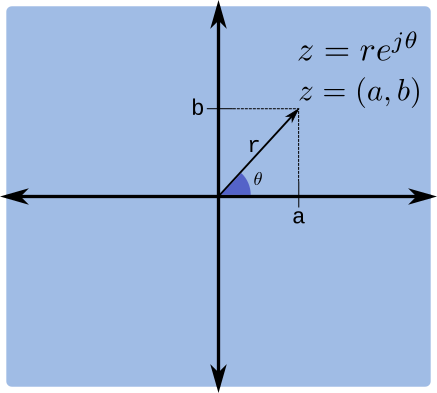
\includegraphics[width=.23\textwidth]{../Algebra/Images/complex_numbers.png}
\subsection{Modulo y argumento de un numero complejo}
\begin{defi}
   El modulo de un numero complejo $z=a+bj$ representa su distancia al origen, y se anota: $|z| = +\sqrt{a^{2}+b^{2}}$
\end{defi}
De lo anterior surge que la distancia entre dos puntos en el plano cartesiano $(a,b)$ y $(c,d)$ se puede calcular: $|(a+bj)-(c+dj)|$
\begin{defi}
   El argumento de un numero complejo $z=a+bj$ es el angulo orientado que forma con el semieje positivo de $x$ y por lo tanto tiene $\infty$ argumentos. Basta elegir uno de ellos que lo llamaremos $\theta$ y todos los demas son : $\theta+2k\pi$ con $k=\pm 1, \pm 2, ...$
\end{defi}
Si $|z|=r$ y $Arg[z]=\theta$ entonces llamaremos al par ordenado $(r, \theta)$ a la representacion del numero complejo $z$ en coordenadas polares. Y como $x=r\cos(\theta)$ e $y=r\sin(\theta)$ se conoce como la representacion trigonometrica $z=r(\cos(\theta)+ j\sin(\theta))$.

\begin{defi}{Potencias:}
   Dado un numero complejo $z=r(\cos(\theta)+j\sin(\theta))$ sus potencias son:
   \begin{equation}
      z^{n} = r^{n}(\cos(n\theta)+j\sin(n\theta))
   \end{equation}
\end{defi}


La representacion trigonometrica nos ayuda a entender el producto y el cociente de los numeros complejos.
\begin{align}
   z_{1}z_{2} &= r_{1}(\cos(\theta_{1})+j\sin(\theta_1))r_{2}(\cos(\theta_{2})+j\sin(\theta_{2}))\\
   z_{1}z_{2} &= r_{1}r_{2}[(\cos(\theta_1)\cos(\theta_2)-\sin(\theta_1)\sin(\theta_2))+j(\cos(\theta_1)\sin(\theta_2)+\cos(\theta_2)\sin(\theta_1))]\\
   z_{1}z_{2} &= r_{1}r_{2}[\cos(\theta_1 + \theta_2)+j(\sin(\theta_1 + \theta_2))]
\end{align}

\begin{defi}
   El modulo del producto es el producto de los modulos: $|z_1 z_2|=|z_1||z_2|$
\end{defi}

\begin{defi}
   Un argumento (ya que hay $\infty$) del producto es la suma de los argumentos: $Arg(z_1 z_2)=Arg(z_1)+Arg(z_2)$
\end{defi}

\begin{defi}{Raices n-esimas de la unidad:}
   En general se tienen $n$ raices n-esimas de la unidad, ya que $z^{n} = r^{n}(\cos(n\theta)+j\sin(n\theta))=1$ entonces $r=1$ y $n\theta=2k\pi$
   Tomando sucesivamente $n=0,1,2,3,...,n-1$ encontramos las $n$ raices $\cos(\frac{2k}{n}\pi)+j\sin(\frac{2k}{n}\pi)$ que son potencias sucesivas de:
   $\omega = \cos(\frac{2}{n}\pi)+j\sin(\frac{2}{n}\pi)$. Se disponen como vertices de un poligono regular de $n$ lados inscriptos dentro de la circunferencia unidad
\end{defi}

\begin{defi}{Raices de un numero:}
   Sea $\omega=r(\cos(\theta)+j\sin(\theta))$ si $z=s(\cos(\theta)+j\sin(\theta))$ es una raiz n-esima de $\omega$ tenemos:
   $z^{n}=s^{n}(\cos(n\phi)+j\sin(n\phi))=r(\cos(\theta)+j\sin(\theta))$. De donde se obtiene que $s^{n}=r$ entonces $s=r^{1/n}>0$ y 
   $n\phi=\theta + 2k\pi$ con $k$ entero.
   
   Luego: $\phi=\frac{\theta}{n}+\frac{2k\pi}{n}$ con $k=0,\pm 1,\pm 2,\pm 3...,\pm (n-1)$. para $k=0,1,2,3,...,n-1$ obtenemos $n$ raices distintas:

   \begin{equation}
      z_{k}=r^{1/n}(\cos(\frac{\theta + 2k\pi}{n})+j\sin(\frac{\theta + 2k\pi}{n}))
   \end{equation}
\end{defi}

%--------------------------------------------------------------------------
% @file polynomials.tex
%
% @date 09/20/16 16:22:57
% @author Martin Noblia
% @email martin.noblia@openmailbox.org
%
% @brief
% Breve resumen de polinomios
% @detail
%
% Licence:
% This program is free software: you can redistribute it and/or modify
% it under the terms of the GNU General Public License as published by
% the Free Software Foundation, either version 3 of the License, or (at
% your option) any later version.
% 
% This program is distributed in the hope that it will be useful, but
% WITHOUT ANY WARRANTY; without even the implied warranty of
% MERCHANTABILITY or FITNESS FOR A PARTICULAR PURPOSE.  See the GNU
% General Public License for more details.
% 
% You should have received a copy of the GNU General Public License
%
%---------------------------------------------------------------------------
\section{Polinomios}
\begin{defi}{Polinomios:}
   Un polinomio en la variable $x$ es de la forma $a_0 + a_1 x + a_2 x^2 + a_3 x^3 + ... + a_n x^n$
\end{defi}
\begin{defi}
   Dos polinomios son iguales si los coeficientes de igual grado son iguales: Sean $p(x) = a_0 + a_1 x + a_2 x^2 + a_3 x^3 + ... + a_n x^n$ y 
   $q(x) = b_0 + b_1 x + b_2 x^2 + b_3 x^3 + ... + b_n x^n$ entonces decimos que $p(x) = q(x)$ si y solo si:
   \begin{align}
      a_0 &= b_0\\
      a_1 &= b_1\\
      a_2 &= b_2\\
      a_3 &= b_3\\
      .\\
      .\\
      .\\
      a_n &= b_n
   \end{align}
\end{defi}

\begin{teo}{Teorema del resto:}
   Al dividir un polinomio $p(x)$ por $x-a$ se obtiene como resto $p(a)$
\end{teo}
\begin{teo}
   Un polinomio de grado $n$ no puede tener mas de $n$ raices distintas
\end{teo}

\begin{teo}{Principio de identidad de Polinomios:}
   Si dos polinomios de grado $\leq n$ valen lo mismo en $n+1$ puntos distintos entonces son iguales
\end{teo}
 \begin{teo}{Criterio de Gauss:}
    Sea $\frac{p}{q}$ una raiz racional del polinomio con coeficientes enteros: $z(x) = a_0 + a_1 x + a_2 x^2 + a_3 x^3 + ... + a_n x^n$
    Si $a_0 a_n \neq 0$ y $p$, $q$ son coprimos entonces $p|a_0$ y $q|a_n$
 \end{teo}

%--------------------------------------------------------------------------
% @file linear_systems.tex
%
% @date 09/26/16 09:33:12
% @author Martin Noblia
% @email martin.noblia@openmailbox.org
%
% @brief
% Resumen de sistemas lineales.
% @detail
%
% Licence:
% This program is free software: you can redistribute it and/or modify
% it under the terms of the GNU General Public License as published by
% the Free Software Foundation, either version 3 of the License, or (at
% your option) any later version.
% 
% This program is distributed in the hope that it will be useful, but
% WITHOUT ANY WARRANTY; without even the implied warranty of
% MERCHANTABILITY or FITNESS FOR A PARTICULAR PURPOSE.  See the GNU
% General Public License for more details.
% 
% You should have received a copy of the GNU General Public License
%
%---------------------------------------------------------------------------
% begin
%---------------------------------------------------------------------------
% Resumen de sistemas lineales
%---------------------------------------------------------------------------
\section{Sistemas Lineales}

\subsection{Matrices}
Una matrix $A$ de tamanio $m \times n$ es un arreglo rectangular de $m \, n$ numeros
dispuestos en $m$ filas y $n$ columnas. Por ejemplo:
$
\begin{bmatrix}
   1 & 0 & 1\\
   0 & 1 & 0 \\
   1 & 3 & 7
 \end{bmatrix}
$
Una matriz generica de tamanio $m \times n$ la anotamos: $A=(a_{ij})$ de tal manera que 
su elemento en la fila $i$ columna $j$ es $a_{ij}$. La fila $i$ de $A$ es:
$
\begin{bmatrix}
   a_{i1} & a_{i2} & a_{i3} & \cdots & a_{i\,n}
 \end{bmatrix}
$
y la columna $j$ de $A$ es:
$
\begin{bmatrix}
   a_{1j} \\ a_{2j} \\ a_{3j} \\ \vdots \\a_{n \, t}
 \end{bmatrix}
$





\end{multicols*}
\end{document}
